\documentclass[a4paper,10pt]{book}

\usepackage[usenames]{color}
\usepackage{bm}
\usepackage{amsmath}
\usepackage{appendix}
\usepackage{xspace}
\usepackage{a4wide}
\usepackage{wrapfig}
\usepackage[numbers,comma,sort&compress]{natbib}
\usepackage{graphicx}
%\usepackage{xstring}
\usepackage{listings,xcolor,courier}
%\usepackage{draftcopy}
\usepackage{longtable}
\usepackage{paralist}
%\usepackage{fancyvrb}
\usepackage{listings}

\definecolor{webgreen}{rgb}{0,.5,0}
\definecolor{webbrown}{rgb}{.6,0,0}
\definecolor{invisiblegray}{rgb}{.97,0.97,0.97}

\usepackage
[dvipdf, %or dvips or pdftex 
pagebackref, %or backref
colorlinks=true,
linkcolor=webgreen, %defined below
filecolor=webbrown, %defined below
citecolor=webgreen, %defined below
pdftitle={VOTCA-CT manual},
pdfauthor={},
pdfsubject={VOTCA-CT},
pdfkeywords={charge transport organic semiconductors},
bookmarksopen=false,
pdfpagemode=UseNone]{hyperref}

%\pdfcompresslevel=9

\usepackage[T1]{fontenc}
%\usepackage{times}
\usepackage{type1cm}

\def\bibsection{%
    \section*{References}%
}

\begin{document}


\lstset{
  language=XML,
  frame=lines,
  backgroundcolor=\color{invisiblegray},
  basicstyle=\ttfamily\footnotesize,
  identifierstyle=\color{red},
  keywordstyle=\color{blue},
  commentstyle=\color{gray}\rmfamily\itshape,
  mathescape=true,
  morekeywords={estatic_params,estatic_method,epsilon_dielectric,s_eps}
}

\newcommand{\equ}[1]{eq.~\eqref{equ:#1}}
\newcommand{\Equ}[1]{Eq.~\eqref{equ:#1}}
\newcommand{\fig}[1]{figure~\ref{fig:#1}}
\newcommand{\Fig}[1]{Figure~\ref{fig:#1}}
\newcommand{\sect}[1]{section~\ref{sec:#1}}

\newcommand{\slink}[2]{\hyperref[sec:#1]{#2}}


\newcommand{\xml}{XML\xspace}
\newcommand{\gromacs}{GROMACS\xspace}
\newcommand{\gaussian}{GAUSSIAN\xspace}
\newcommand{\turbomole}{TURBOMOLE\xspace}
\newcommand{\tinker}{TINKER\xspace}

\newcommand{\Alq}{$\mathrm{Alq}_3$\xspace}
\newcommand{\dcvt}{DCV2T\xspace}

\newcommand{\xyz}{\texttt{geometry.xyz}\xspace}
\newcommand{\orb}{\texttt{zindo.orb}\xspace}
\newcommand{\votcactp}{{\MakeUppercase{votca-ctp}}\xspace}

\newcommand{\calculator}{\hyperref[sec:calculators]{calculator}\xspace}

\newcommand{\xmloptions}{\texttt{options.xml}\xspace}
\newcommand{\xmlcsg}{\texttt{map.xml}\xspace}
\newcommand{\xmlsegments}{\texttt{segments.xml}\xspace}
\newcommand{\sqlstate}{\texttt{state.db}\xspace}
\newcommand{\topology}{\texttt{topol.tpr}\xspace}
\newcommand{\trajectory}{\texttt{traj.xtc}\xspace}

\newcommand{\opt}{\texttt{{ -}-opt}\xspace}
\newcommand{\seg}{\texttt{{ -}-s}\xspace}
\newcommand{\sql}{\texttt{{ -}-db}\xspace}
\newcommand{\exe}{\texttt{{ -}-exec}\xspace}
\newcommand{\tpl}{\texttt{{ -}-top}\xspace}
\newcommand{\csg}{\texttt{{ -}-cg}\xspace}
\newcommand{\trj}{\texttt{{ -}-trj}\xspace}


\newcommand{\refcalc}{\hyperref[ref:calculators]{calculators}\xspace}

\newcommand{\overlap}{\hyperref[prog:moo_overlap]{\texttt{moo\_overlap}}\xspace}
\newcommand{\ctprun}{\hyperref[prog:ctp_run]{\texttt{ctp\_run}}\xspace}
\newcommand{\ctpmap}{\hyperref[prog:ctp_map]{\texttt{ctp\_map}}\xspace}

\newcommand{\ecoulomb}{\hyperref[calc:ecoulomb]{\texttt{ecoulomb}}\xspace}
\newcommand{\dumptraj}{\hyperref[calc:dumptraj]{\texttt{dumptraj}}\xspace}
\newcommand{\integrals}{\hyperref[calc:integrals]{\texttt{integrals}}\xspace}

\newcommand{\suggestion}[1]{{\color{red}SUGGESTION: #1}}

\newcommand{\segmentref}[1]{segments.#1}
\newcommand{\segmentopt}[1]{\hyperlink{\segmentref{#1}}{\StrSubstitute{#1}{_}{\_}}\xspace}
\newcommand{\calcref}[1]{#1}
\newcommand{\calcopt}[1]{\hyperlink{\calcref{#1}}{\StrSubstitute{#1}{_}{\_}}\xspace}

\newcommand{\calc}[1]{\hyperref[calc:#1]{\texttt{#1}}\xspace}



\frontmatter
\begin{titlepage}

%\center{\fontsize{4cm}{5cm}\selectfont VOTCA-CT}
%\center{\fontsize{1.5cm}{3cm}\selectfont USER MANUAL}

\center{\huge \sc VOTCA-CTP \\ \vspace*{1cm} Charge Transport Simulations}
\vspace*{1cm}
\center{\Large \sc User Manual}

\vspace*{3cm}
\center{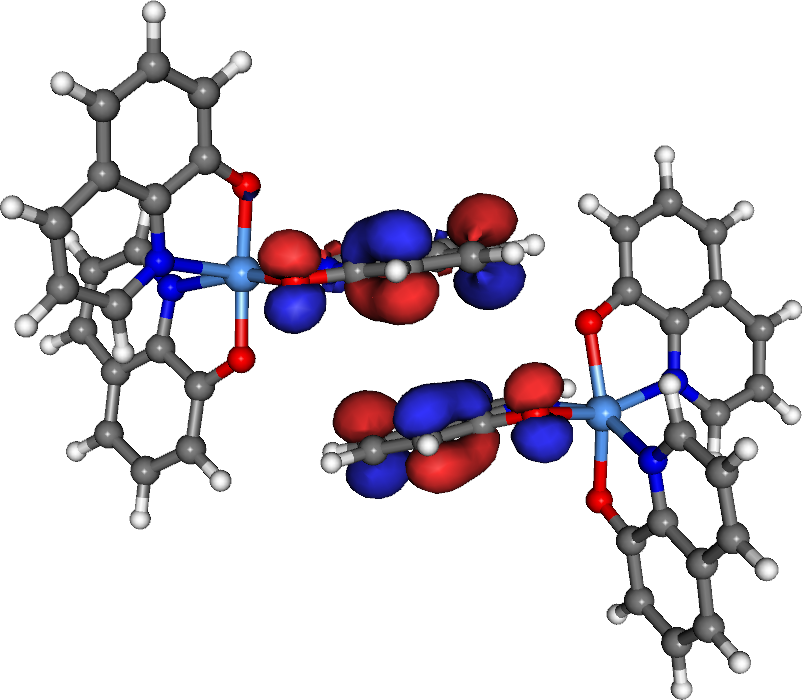
\includegraphics[width=0.6\columnwidth]{fig/logo}}
\vspace*{1cm}
\vfill

\center{\footnotesize{compiled from: \hgid}}
%\center{\footnotesize{Programs version: \refhgid}}
%\vspace*{1cm}
%\center{
%\large{\copyright \hspace*{0.1cm} VOTCA development team}
%}
\vspace*{0.5cm}
\center{\large{\today}} \\
\vspace*{0.3cm}
\htmladdnormallink{\color{black}\large{www.votca.org}}{http://www.votca.org}
\end{titlepage}

\section*{Disclamer}
The best way to start using the software is to look at provided tutorials. The reference section is generated automatically from the source code, so please make sure that your software and manual versions match.  

\section*{Citations}
Development of this software depends on academic research grants. If you are using the package, please cite the  following papers \\

\vspace{0.1cm}
\noindent
\cite{poelking_long-range_2016} Long-range embedding of molecular ions and excitations in a polarizable molecular environment, \\
Carl Poelking and Denis Andrienko \\
\htmladdnormallink{  {\itshape J. Chem. Theory Comp.} 12, 4516-4523, 2016}
{http://dx.doi.org/10.1021/acs.jctc.6b00599} \\

\vspace{0.1cm}
\noindent
\cite{ruhle_microscopic_2011} Microscopic simulations of charge transport in disordered organic semiconductors, \\
Victor R\"uhle, Alexander Lukyanov, Falk May, Manuel Schrader, Thorsten Vehoff, James Kirkpatrick, Bj\"orn Baumeier and Denis Andrienko \\
\htmladdnormallink{  {\itshape J. Chem. Theor. Comp.} 7, 3335, 2011}
{http://dx.doi.org/10.1021/ct200388s} \\

\vspace{0.1cm}
\noindent
\cite{ruhle_versatile_2009} Versatile Object-oriented Toolkit for Coarse-graining Applications \\
Victor R\"uhle, Christoph Junghans, Alexander Lukyanov, Kurt Kremer and Denis Andrienko \\
\htmladdnormallink{  {\itshape J. Chem. Theor. Comp.} 5, 3211, 2009}
{http://dx.doi.org/10.1021/ct900369w}

\section*{Development}
The core development is currently taking place at the Max Planck Institute for Polymer Research, Mainz, Germany.

\section*{Copyright}
\votcactp is free software. The entire package is available under the Apache License. For details, check
the LICENSE file in the source code. The \votcactp source code is available on our homepage, \htmladdnormallink{\color{black}www.votca.org}{http://www.votca.org}.

\vfill

\thispagestyle{empty}
\cleardoublepage

\tableofcontents
%\cleardoublepage
\mainmatter
\chapter{Introduction}
\label{sec:introduction}

Charge carrier dynamics in an organic semiconductor can often be described in terms of charge hopping between localized states. The hopping rates depend on \slink{sec:transfer_integrals}{electronic coupling elements}, \slink{sec:reorganization}{reorganization energies}, and \slink{sec:site_energies}{site energies}, which vary as a function of position and orientation of the molecules. 
%The exact evaluation of these contributions in a molecular assembly is computationally prohibitive. Various, often semi-empirical, approximations are employed instead. 
The purpose of the \votcactp package~\cite{ruhle_microscopic_2011} is to simplify the workflow for charge transport simulations, provide a uniform error-control for the methods, flexible platform for their development, and eventually allow {\em in silico} prescreening of organic semiconductors for specific applications. 

The toolkit is implemented using modular concepts introduced earlier in the Versatile Object-oriented Toolkit for Coarse-graining Applications (VOTCA)~\cite{ruhle_versatile_2009}. It contains different \slink{sec:programs}{programs}, which execute specific tasks implemented in \slink{sec:calculators}{calculators} representing an individual step in the workflow. \Fig{summary} summarizes a typical chain of commands to perform a charge transport simulation:   
%
First, the VOTCA code structures are adap\-ted to reading atomistic trajectories, mapping them onto \slink{segments}{conjugated segments and rigid fragments}, and substituting (if needed) rigid fragments with the optimized copies (\ctpmap). The programs \ctprun and \ctpparallel (for heavy-duty tasks) are then used to calculate all bimolecular charge hopping rates (via precalculation of all required ingredients). \slink{sec:site_energies}{Site energies (or energetic disorder)} can be determined as a combination of internal (ionization potentials/electron affinities of single molecules) as well as electrostatic and polarization contributions with in the molecular environment. The calculation of \slink{sec:transfer_integrals}{electronic coupling elements} between conjugated segments from the corresponding molecular orbitals can be performed using a \slink{sec:dipro}{dimer-projection} technique based on \slink{sec:dft}{density-functional} theory (DFT). This requires explicit calculations using quantum-chemistry software for which we provide interfaces to \gaussian, \turbomole, and \nwchem. Alternatively, the \slink{sec:izindo}{molecular orbital overlap} module calculates electronic coupling elements relying on the semi-empirical INDO Hamiltonian and molecular orbitals in the format provided by the \gaussian package. 

The  \slink{sec:kmc}{kinetic Monte Carlo} module reads in the \slink{neighborlist}{neighbor list}, \slink{morphology}{site coordinates}, and \slink{rates}{hopping rates} and performs charge dynamics simulations using either periodic boundary conditions or charge sources and sinks. 

The toolkit is written as a combination of modular C++ code and scripts. The data transfer between programs is implemented via a \slink{statefile}{state file} (sql database), which is also used to restart simulations. Analysis functions and most of the calculation routines are encapsulated by using the observer pattern~\cite{gamma_design_1995} which allows the implementation of new functions as individual modules.

In the following \sect{theory}, we summarize the \slink{sec:theory}{theoretical background} of the workflow of charge transport simulations and i partciular its individual steps. \Sect{io} describes the structure and content of input and output files, while a full reference of \slink{sec:programs}{programs} and \slink{sec:calculators}{calculators} is available in \sect{reference}. For a hands-on tutorial, the reader is referred to the \hyperref[http://code.google.com/p/votca-ctp/]{\votcactp} project page at http://code.google.com/p/votca-ctp/.



\tikzstyle{decision} = [diamond, draw, fill=mygray]
\tikzstyle{line} = [draw, -stealth, thick]
\tikzstyle{block} = [draw, rectangle, fill=mygray, text width=0.5\linewidth]
\tikzstyle{smallblock} = [draw, rectangle, fill=mygray, text width=0.4\linewidth]
\tikzstyle{info} = [text width=0.35\linewidth]
\tikzstyle{smallinfo} = [text width=0.25\linewidth]
\tikzstyle{biginfo} = [text width=0.9\linewidth]
\begin{figure}
\centering
\newcommand{\vgap}{0.5cm}
\begin{scriptsize}
\noindent\begin{tikzpicture}
\node [block] (mapping) {{\bf Mapping}\\Converts and partitions atomistic \gromacs trajectory \vskip 0.1cm
{\noindent  \cmdmap}
\vskip 0.1cm};

\node[smallinfo, left=0.0 of mapping] (input) {{\bf Input files:}\\\texttt{conf.gro}\\\,\hskip 0.1cm\gromacs trajectory\\\texttt{topol.tpr}\\\hskip0.1cm\gromacs topology\\\texttt{\xmlcsg}\\\hskip0.1cm mapping and energies\\\texttt{options.xml}\\\hskip0.1cm options for \slink{sec:calculators}{calculators}\vskip 0.2cm {\bf Output files:}\\\texttt{\sqlstate}\\\hskip0.1cm \sqlite database file for\\\hskip0.1cm data transfer between\\\hskip0.1cm modules};

\node [block, below=\vgap of mapping] (nbl) {{\bf Neighbor list}\\Indentifies close molecular pairs between which charge transfer rates will be calculated \vskip 0.1cm
{\noindent \cmdnbl}
\vskip 0.1cm};


\node [block, below=\vgap of nbl] (site_energies) {{\bf Site energies}\\Calculates electrostatic and polarization contribution to site energies \vskip 0.1cm
{\noindent  \cmdemlt} };

\node [block, below=\vgap of site_energies] (int_energies) {{\bf Internal site and reorganization energies}\\Imports internal site energy (IP, EA) and reorganization energies for charging and discharging to \sqlstate \vskip 0.1cm
{\noindent  \cmdeint}
\vskip 0.1cm};


% above right=0.7cm and 4cm of A
\node[decision, below=\vgap of int_energies](decision1){Transfer integrals};

%\node (AuxNode01) [text width=6em, below of = decision1, node distance=7em ] {};

\node [smallblock, below left=\vgap of decision1] (DFT_TI) {{\bf Monomers with DFT}\\Calculate the relevant transport orbitals of monomers \vskip 0.1cm
{ \cmdedft \job\, ''\wrt \run'' }};

\node [smallblock, below=\vgap of DFT_TI] (DFT_TI2) {{\bf Transfer integrals with DFT}\\Calculate electronic coupling elements for all pairs in the neighbor list \vskip 0.1cm
{ \cmdidft \job\, ''\wrt \run \rd'' }
\vskip 0.1cm};

\node [smallblock, below right=\vgap of decision1] (DFT_ZINDO) {{\bf Transfer integrals with ZINDO}\\Calculate electronic coupling elements for all pairs in the neighbor list  \vskip 0.1cm
{\noindent  \cmdizindo }
\vskip 0.1cm};


\node[info, below=0.2cm of DFT_ZINDO] (ti_info) {{One can choose between quantum-chemical (computationally expensive) or semi-empirical (fast, but not always sufficiently accurate) evaluation of transfer integrals.}};

\node (AuxNode01) [below=\vgap of DFT_TI2, xshift=0.25\linewidth] {};


\node [block, below=\vgap of DFT_TI2, xshift=0.275\linewidth] (outer_reorg) {{\bf Outersphere reorganization energies}\\Contribution to reorganization of surrounding molecules due to polarization. (optional for Marcus rates)  \vskip 0.1cm
{\noindent  \cmdouter}
\vskip 0.1cm};

\node [block, below=\vgap of outer_reorg] (rates) {{\bf Charge transfer rates}\\Calculates rates for charge transfer among all pairs in the neighborlist \vskip 0.1cm
{\noindent \cmdrates}
};

\node [block, below=\vgap of rates] (kmc) {{\bf Charge dynamics via kMC}\\Hopping of charge carriers simulated via kinetic Monte Carlo \vskip 0.1cm
{\noindent \cmdkmc }
};

\node [biginfo, below=\vgap of kmc] (calc) {{\noindent Get list of available calculators: \ctprun/\ctpparallel/\kmcrun  \texttt{ -l}}\\ Get help and list of options for a calculator: \ctprun/\ctpparallel/\kmcrun  \texttt{ -d }\calc{neighborlist}};

\path [line] (mapping) -- (nbl);
\path [line] (nbl) -- (site_energies);
\path [line] (site_energies) -- (int_energies);
\path [line] (int_energies) -- (decision1);
\path [line] (DFT_TI) -- (DFT_TI2);
\path [line] (decision1) -| node[yshift=0.5em, xshift=1em] {DFT} (DFT_TI);
\path [line] (decision1) -| node[yshift=0.5em, xshift=-1em] {ZINDO} (DFT_ZINDO);
\path [line] (DFT_TI2.east) -| (outer_reorg.north);
\path [line] (DFT_ZINDO.west) -| (outer_reorg);
\path [line] (outer_reorg) -- (rates);
\path [line] (rates) -- (kmc);
\end{tikzpicture}


\end{scriptsize}
\caption{A practical workflow of charge transport simulations using \votcactp. The \slink{sec:theory}{theoretical background} of the individual steps is given in \sect{theory}. \Sect{io} describes the content of input and output files, while a full reference of \slink{sec:programs}{programs} and \slink{sec:calculators}{calculators} is available in \sect{reference}.  }
\label{fig:summary}
\end{figure}
\chapter{Theoretical background}
\label{sec:theory}

\section{Workflow}
\label{sec:wokflow}

A typical workflow of charge transport simulations is depicted in \fig{workflow}. The first step is the simulation of an \slink{morphology}{atomistic morphology}, which is then partitioned on \slink{segments}{hopping sites}. The coordinates of the hopping sites are used to construct a list of pairs of molecules, or \slink{neighborlist}{neighbor list}. 

\begin{figure}[h]
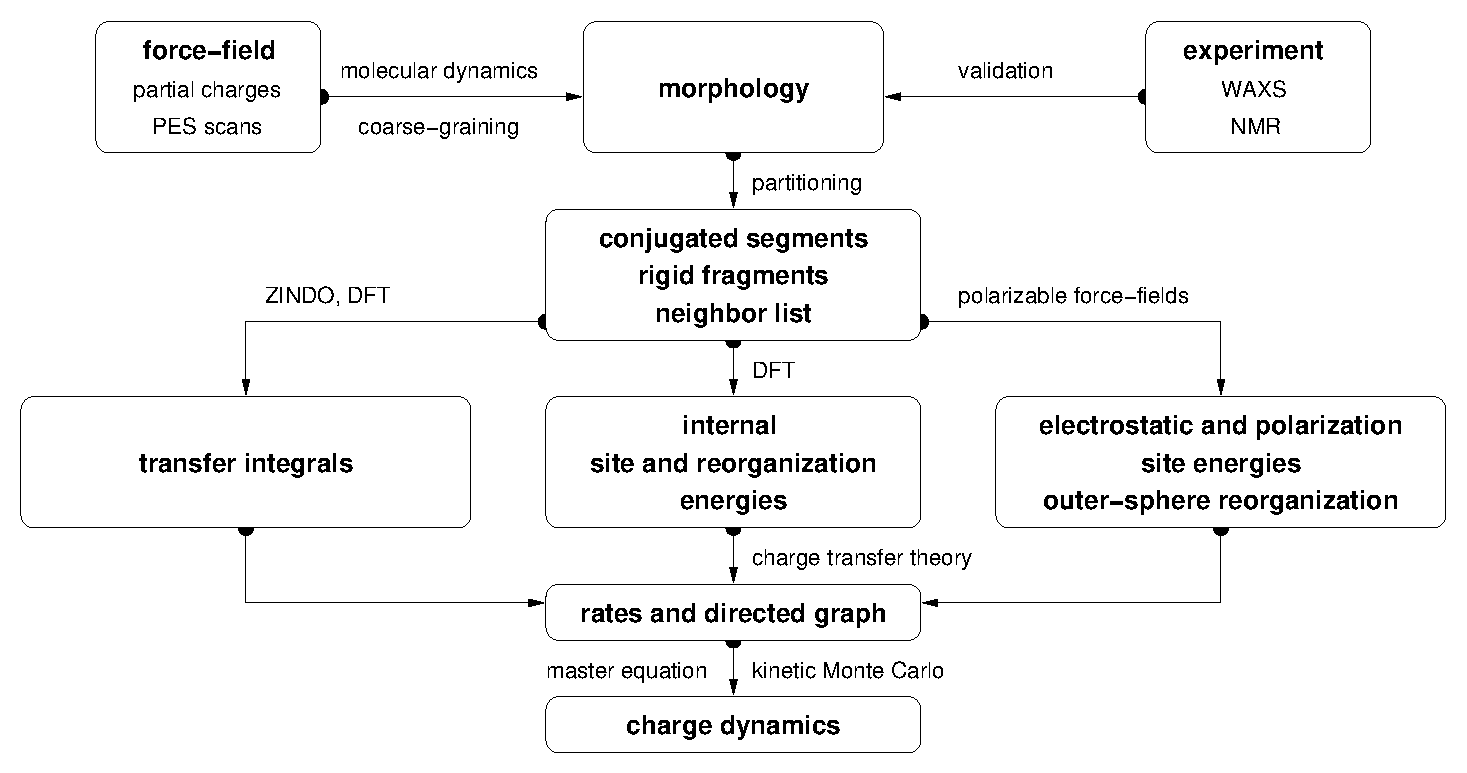
\includegraphics[width=\textwidth]{fig/workflow/workflow}
 \caption{%
   Workflow for microscopic simulations of charge transport.  %
   \label{fig:workflow}}
\end{figure}

For each pair an \slink{transfer_integrals}{electronic coupling element}, a \slink{reorganization}{reorganization energy}, a \slink{site_energies}{driving force}, and eventually the \slink{rates}{hopping rate} are evaluated. The neighbor list and hopping rates define a directed graph. The corresponding master equation is solved using the \slink{kmc}{kinetic Monte Carlo} method, which allows to explicitly monitor the charge dynamics in the system as well as to calculate time or ensemble averages of occupation probabilities, charge fluxes, correlation functions, and field-dependent mobilities.


\begin{figure}[p]
\includegraphics[width=\textwidth]{fig/workflow_practical/workflow_practical}
 \caption{%
   Workflow for microscopic simulations of charge transport including calls.  %
   \label{fig:workflow}}
\end{figure}


\tikzstyle{decision} = [diamond, draw, fill=blue!50]
\tikzstyle{line} = [draw, -stealth, thick]
\tikzstyle{elli}=[draw, ellipse, fill=red!50,minimum height=8mm, text width=5em ]
\tikzstyle{block} = [draw, rectangle, fill=blue!50, text width=\linewidth]
\tikzstyle{smallblock} = [draw, rectangle, fill=blue!50, text width=0.4\linewidth]
\begin{figure}
\centering
\newcommand{\vgap}{0.5cm}
\begin{footnotesize}
\noindent\begin{tikzpicture}
\node [block] (mapping) {{\bf Mapping}\\Converts and partitions atomistic \gromacs trajectory \vskip 0.1cm
{\noindent  \ctpmap \tpl \topology \trj \trajectory \seg \xmlcsg  \sql \sqlstate}
\vskip 0.1cm};

\node [block, below=\vgap of mapping] (nbl) {{\bf Neighbor list}\\Indentifies close molecular pairs between which charge transfer rates will be calculated \vskip 0.1cm
{\noindent  \ctprun \opt \xmloptions  \seg  \xmlsegments \sql  \sqlstate \exe  \calc{neighborlist}}
\vskip 0.1cm};


\node [block, below=\vgap of nbl] (site_energies) {{\bf Site energies}\\Calculates electrostatic and polarization contribution to site energies \vskip 0.1cm
{\noindent  \ctprun \opt \xmloptions  \sql  \sqlstate \exe  \calc{emultipole} } };

\node [block, below=\vgap of site_energies] (int_energies) {{\bf Internal site and reorganization energies}\\Imports internal site energy (IP, EA) and reorganization energies for charging and discharging to \sqlstate \vskip 0.1cm
{\noindent  \ctprun \opt \xmloptions  \sql  \sqlstate \exe  \calc{einternal} }
\vskip 0.1cm};


% above right=0.7cm and 4cm of A
\node[decision, below=\vgap of int_energies](decision1){Transfer integrals};

%\node (AuxNode01) [text width=6em, below of = decision1, node distance=7em ] {};

\node [smallblock, below left=\vgap of decision1] (DFT_TI) {{\bf Monomers with DFT}\\Calculate the relevant transport orbitals of monomers\\ prepare job file \vskip 0.1cm
{ \ctpparallel \opt \xmloptions \sql \sqlstate \exe \calc{edft} \job \wrt }
\vskip 0.1cm execute jobs \vskip 0.1cm
{ \ctpparallel \opt \xmloptions \sql \sqlstate \exe \calc{edft} \job \run }
};

\node [smallblock, below=\vgap of DFT_TI] (DFT_TI2) {{\bf Electronic coupling with DFT}\\Calculate electronic coupling elements for all pairs in the neighbor list \vskip 0.1cm
{ \ctpparallel \opt \xmloptions \sql \sqlstate \exe \calc{idft} \job `` \wrt \run \rd\'' }
\vskip 0.1cm};

\node [smallblock, below right=\vgap of decision1] (DFT_ZINDO) {{\bf Electronic coupling with ZINDO}\\Imports internal site energy (IP, EA) and reorganization energies for charging and discharging to \sqlstate \vskip 0.1cm
{\noindent  \ctprun \opt \xmloptions  \sql  \sqlstate \exe  \calc{einternal} }
\vskip 0.1cm};

\node (AuxNode01) [below=\vgap of DFT_TI2, xshift=0.25\linewidth] {};


\node [block, below=\vgap of DFT_TI2, xshift=0.275\linewidth] (outer_reorg) {{\bf Outersphere reorganization energies}\\Imports internal site energy (IP, EA) and reorganization energies for charging and discharging to \sqlstate \vskip 0.1cm
{\noindent  \ctprun \opt \xmloptions  \sql  \sqlstate \exe  \calc{outersphere} }
\vskip 0.1cm};

\node [block, below=\vgap of outer_reorg] (rates) {{\bf Charge transfer rates}\\Calculates rates for charge transfer among all pairs in the neighborlist \vskip 0.1cm
{\noindent \small \ctprun \opt \xmloptions \sql  \sqlstate \exe  \calc{rates} }
};

\node [block, below=\vgap of rates] (kmc) {{\bf Charge dynamics via kMC}\\Hopping of charge carriers simulated via kinetic Monte Carlo \vskip 0.1cm
{\noindent  \kmcrun \opt \xmloptions  \sql  \sqlstate \exe  \calc{kmcmultiple} }
};
%%
%(ClOp.west) -- ++(-0.2,0) -- ([yshift=0.5cm, xshift=-0.2cm] Pressure.north west) -|
%     ([xshift=-1cm]Sensor.south);
%    \draw[myarrow] (Ammeter.east) -- ++(0.2,0) -- ([yshift=0.5cm, xshift=0.2cm] Temperature.north east) -|
%     ([xshift=1cm]Sensor.south);

%\node [block, left of=mapping, xshift=-5em] (nbl) {Process 1};
%\node [elli, above of=mapping, yshift=5em] (user) {user};
%\node [block, right of=mapping, xshift=5em] (process2) {Process 2};
%\node[decision, below of=mapping, yshift=-5em](decision1){Process 1?};
%arrows
%\path [line] (user) -- (mapping);
\path [line] (mapping) -- (nbl);
\path [line] (nbl) -- (site_energies);
\path [line] (site_energies) -- (int_energies);
\path [line] (int_energies) -- (decision1);
\path [line] (DFT_TI) -- (DFT_TI2);
\path [line] (decision1) -| node[yshift=0.5em, xshift=1em] {DFT} (DFT_TI);
\path [line] (decision1) -| node[yshift=0.5em, xshift=-1em] {ZINDO} (DFT_ZINDO);
\path [line] (DFT_TI2) -- (outer_reorg);
\path [line] (DFT_ZINDO) -- (outer_reorg);
\path [line] (outer_reorg) -- (rates);
\path [line] (rates) -- (kmc);
\end{tikzpicture}


\end{footnotesize}
\caption{LALA}
\end{figure}


\section{Material morphology}
\label{sec:morphology}

There is no generic recipe on how to predict a large-scale atomistically-resolved morphology of an organic semiconductor. The required methods are system-specific: for ultra-pure crystals, for example, density-functional methods can be used provided the crystal structure is known from experiment. For partially disordered organic semiconductors, however, system sizes much larger than a unit cell  are required. Classical molecular dynamics or Monte Carlo techniques are then the methods of choice. 

In molecular dynamics, atoms are represented by point masses which interact via empirical potentials prescribed by a force-field. Force-fields are parametrized for a limited set of compounds and their refinement is often required for new molecules. In particular, special attention shall be paid to torsion potentials between successive repeat units of conjugated polymers or between functional groups and the $\pi$-conjugated system. First-principles methods can be used to characterize the missing terms of the potential energy function. 

Self-assembling materials, such as soluble oligomers, discotic liquid crystals, block copolymers, partially crystalline polymers, etc., are the most complicated to study. The morphology of such systems often has several characteristic length scales and can be kinetically arrested in a thermodynamically non-equilibrium state. For such systems, the time- and length-scales of atomistic simulations might be insufficient to equilibrate or sample desired morphologies. In this case, systematic coarse-graining can be used to enhance sampling~\cite{ruehle_versatile_2009}. Note that the coarse-grained representation must reflect the structure of the atomistic system and allow for back-mapping to the atomistic resolution.

Here we assume that the morphology is already known, that is we know how the topology and the coordinates of all atoms in the systems at a given time. \votcact can read standard \gromacs topology files. Custom definitions of \hyperref[sec:atomistic]{atomistic topology} via \xml files are also possible. Since the description of the atomistic topology is the first step in the charge transport simulations, it is important to follow simple conventions on how the system is partitioned on molecules, residues, and how atoms are named in the topology. Required input files are described in section \hyperref[sec:atomistic]{Atomistic topology}. 


\section{Conjugated segments and rigid fragments}
\label{sec:conjugated_segments}

\begin{wrapfigure}{ht}{0.5\linewidth}
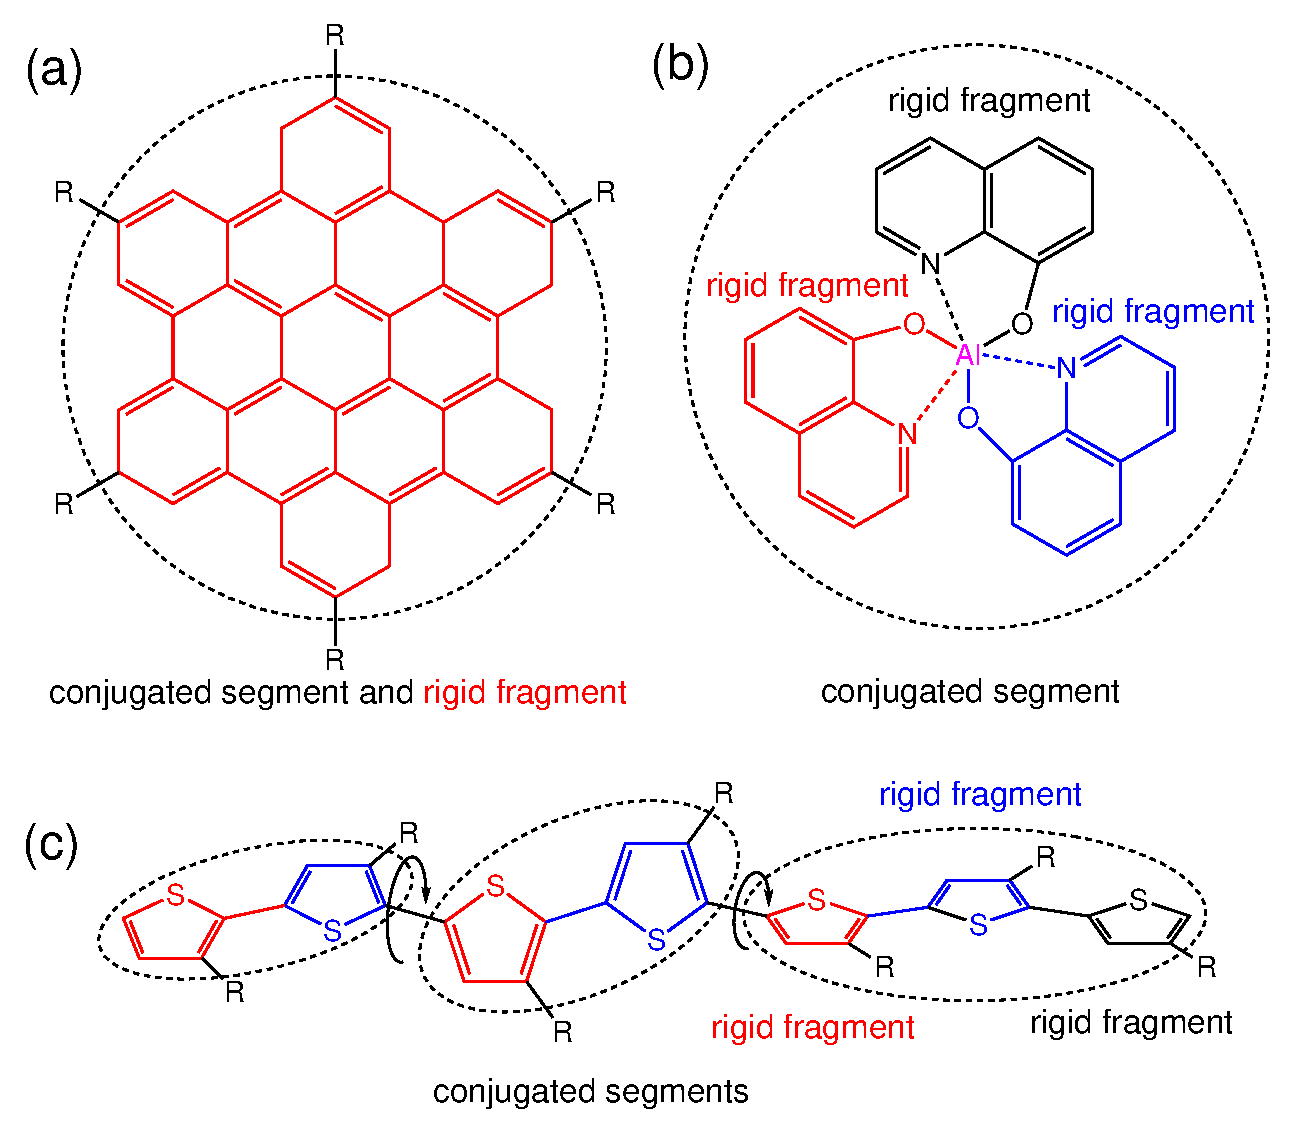
\includegraphics[width=\linewidth]{fig/conjugated_segment/fragment_segment}
\caption{\footnotesize The concept of conjugated segments and rigid fragments. Dashed lines indicate conjugated segments while colors denote rigid fragments. (a) Hexabenzocoronene: the $\pi$-conjugated system is both a rigid fragment and a conjugated segment. (b) \Alq: the Al atom and each ligand are rigid fragments while the whole molecule is a conjugated segment. (c) Polythiophene: each repeat unit is a rigid fragment. A conjugated segment consists of one or more rigid fragments. One molecule can have several conjugated segments.}
\label{fig:segment}
\end{wrapfigure}

With the morphology at hand, the next step is partitioning the system on hopping sites, or conjugated segments, and calculating charge transfer rates between them. Physically intuitive arguments can be used for the partitioning,  which reflects the localization of the wave function of a charge. For most organic semiconductors, the molecular architecture includes relatively rigid, planar $\pi$-conjugated systems, which we will refer to as rigid fragments. A conjugated segment can contain one or more of such rigid fragments, which are linked by bonded degrees of freedom. The dynamics of these degrees of freedom evolves on timescales much slower than the frequency of the internal promoting mode. In some cases, e.g. glasses, it can be `frozen' due to non-bonded interactions with the surrounding molecules.

To illustrate the concept of conjugated segments and rigid fragments, three representative molecular architectures are shown in \fig{segment}. The first one is a typical discotic liquid crystal, hexabenzocoronene. It consists of a conjugated core to which side chains are attached to aid self-assembly and solution processing. In this case the orbitals localized on side chains do not participate in charge transport and the conjugated $\pi$-system is both, a rigid fragment and a conjugated segment. 
%
In \Alq, a metal-coordinated compound, a charge carrier is delocalized over all three ligands. Hence, the whole molecule is one conjugated segment. Individual ligands are relatively rigid, while energies of the order of $k_\text{B}T$ are sufficient to reorient them with respect to each other. Thus the Al atom and the three ligands are rigid fragments.
%
In the case of a conjugated polymer, one molecule can consist of several conjugated segments, while each backbone repeat unit is a rigid fragment. Since the conjugation along the backbone can be broken due to large out-of-plane twists between two repeat units, an empirical criterion, based on the dihedral angle, can be used to partition the backbone on conjugated segments~\cite{ruehle_multiscale_2010}. However, such intuitive partitioning is, to some extent, arbitrary and shall be validated by other methods~\cite{vukmirovi_charge_2008,vukmirovi_charge_2009,mcmahon_ad_2009}. 

After partitioning, an additional step is often required to remove bond length fluctuations introduced by molecular dynamics simulations, since they are already integrated out in the derivation of the rate expression. This is achieved by substituting respective molecular fragments with  rigid, planar $\pi$-systems optimized using first-principles methods. Centers of mass and gyration tensors are used to align rigid fragments, though a custom definition of local axes is also possible. Such a procedure also minimizes discrepancies between the force-field and first-principles-based ground state geometries of conjugated segments, which might be important for calculations of electronic couplings, reorganization energies, and intramolecular driving forces. 

Finally, a list of neighboring conjugated segments is constructed. Two segments are added to this list if the distance between centers of mass of {\em any} their rigid fragments is below a certain cutoff. This allows neighbors to be selected on a criterion of minimum distance of approach rather than center of mass distance, which is useful for molecules with anisotropic shapes.


In addition to coordinates and atom tyoes, the code needs to know how the system is partitioned on  \hyperref[sec:conjugated_segments]{conjugated segments}, which represent localized electronic states available for mobile carriers. 


\section{Neighbor list}
\label{sec:neighborlist}

A list of neigboring molecules (neighbor list) containes all pairs of molecules for which rates (coupling elements, reorganization energies, and site energy differences are evaluated).

Two segments are added to this list if the distance between centers of mass of any of their rigid fragments is below
a certain cutoff. This allows neighbors to be selected on a criterion of minimum distance of approach rather than center of
mass distance, which is useful for molecules with anisotropic shapes.

The neighbor list can be generated from the atomistic trajectory by using the \calc{neighborlist} \calculator. This calculator requires a cutoff, which can be specified in the \xmloptions file. The list is saved to the \sqlstate file:

{\small \ctprun \opt \xmloptions  \seg  \xmlsegments \sql  \sqlstate \exe  \calc{neighborlist} }


\section{Electronic coupling elements}
\label{sec:transfer_integrals}
\subsection{Semi-empirical methods}
\label{sec:moo}

\newcommand{\moo}{MOO\xspace}
\index{electronic coupling!ZINDO}

An approximate method based on Zerner's Independent Neglect of Differential Overlap (ZINDO) has been described in Ref.~\cite{kirkpatrick_approximate_2008}. This semiempirical method is substantially faster than first-principles approaches, since it avoids the self-consistent calculations on each individual monomer and dimer. This allows to construct the matrix elements of the ZINDO Hamiltonian of the dimer from the weighted overlap of molecular orbitals of the two monomers. Together with the introduction of rigid segments, only a single self-consistent calculation on one isolated conjugated segment is required. All relevant molecular overlaps can then be constructed from the obtained molecular orbitals. This Molecular Orbital Overlap (MOO) method has been applied successfully to study charge transport, for instance, in discotic liquid crystals~\cite{kirkpatrick_columnar_2008,marcon_understanding_2009,feng_towards_2009},
polymers~\cite{ruehle_multiscale_2010}, or partially disordered organic crystals~\cite{vehoff_charge_2010-1,vehoff_charge_2010-2,vehoff_charge_2010}.

The main advantage of the molecular orbital overlap \moo library is {\em fast} evaluation of electronic coupling elements. A detailed description of the method is provided in ref.~\cite{kirkpatrick_approximate_2008}. Please site this paper if you are using the method. Note that \moo is based on the semi-empirical ZINDO Hamiltonian and therefore has limited applicability. The general advice is to first compare the accuracy of the \moo method to the DFT-based calculations. 

\moo can be used both in a sandalone mode and as a \calculator of the \votcactp. \moo constructs the Fock operator of a dimer from the  molecular orbitals of monomers by translating and rotating the orbitals and therefore requires the optimized geometry of the molecule and the projection coefficients of the molecular on atomic orbitals. 


\subsubsection{Standalone mode}
For a standalone mode program \overlap is provided 
\begin{verbatim}
 moo_overlap --conjseg benzene.xml --pos1 benzene1.pos --pos2 benzene2.pos
\end{verbatim}
Its input requires a description of two conjugated segments (\texttt{benzene.xml}, positions and orientations of the molecules and the files with molecular coordinates and orbitals. The structure of the files is shown in listings \ref{list:benzene_xml} and  \ref{list:benzene_pos}.
\vskip 0.1cm
\lstinputlisting[
  language=XML,
  label=list:benzene_xml,
  stringstyle=\ttfamily\footnotesize,
  showstringspaces=false,
  caption={\small \texttt{benzene.xml} file with the description of the benzene molecule, which is also a single conjugated segment and a rigid fragment.}] {./programs/benzene.xml}

\vskip 0.1cm

\lstinputlisting[
  language=XML,
  label=list:benzene_pos, 
  stringstyle=\ttfamily\footnotesize,
  showstringspaces=false,
  caption={\small \texttt{benzene1.pos} file which describes the position and orientation of the molecule. The name of the molecule is followed by three coordinates (relative to the center of mass of the supplied \texttt{xyz} file and then by nine elements of the rotation matrix $a_{ij} = e_i e^\text{mol}_j $. The reference coordinate frame is determined from the provided \texttt{xyz} file.}] {./fig/moo/moo_overlap/benzene1.pos}


\subsubsection{Calculator of \votcactp}
Semi-empirical method of evaluation of electronic couplings in a morphology is provided by the \integrals \calculator. In addition to definitions of conjugated segments, atomistic trajectory, and state file, the program needs coordinates and orbitals of conjugated segments. Coordinates are stored in \xyz files with four columns, first being the atom type and the next three atom coordinates. This is a standard \texttt{xyz} format without a header. Note that the atom order in \xyz files can be different from that of the mapping files. The correspondence between the two is established in the file which defines conjugated segments.

\subsection{Density-functional methods}
\label{sec:dft}
\index{electronic coupling!DFT}
While the use of the semiempirical ZINDO method provides an efficient on-the-fly technique to determine electronic coupling elements, it is not generally applicable to all systems. For instance, its predictive capacity with regards to atomic composition and localization behavior of orbitals within more complex structures is reduced. Moreover, transition- or semi-metals are often not even parametrized. In this case, {\it ab-initio} based approaches, e.g., density-functional theory can remedy the situation~\cite{huang_intermolecular_2004,huang_validation_2005,valeev_effect_2006,yin_balanced_2006,yang_theoretical_2007,baumeier_density-functional_2010}. Within the dimer projection method described in detail in Ref.~\cite{baumeier_density-functional_2010}, explicit quantum-chemical calculations are required for every molecule and every hopping pair in the morphology. As a consequence, this procedure is significantly more computationally demanding. The code currently contains scripts which support evaluation of transfer integrals from quantum-chemical calculations performed with the \gaussian and \turbomole packages.

Apart from semi-empirical methods, we also provide interfaces for a DFT-based evaluation of electronic coupling elements. The interfacing procedure consists of three main steps: generation of directory structures containing input coordinates for monomers and dimers, performing the actual quantum-chemical calculations and calculating the transfer integrals using the DIPRO method, and finally reading the output into VOTCA\_CT.

\subsubsection{Generation of directory structure and input coordinates}
First, hopping sites and a neighbor list need to be generated from the atomistic topology and trajectory. Rigid fragments are resubstituted into the molecular geometries and the neighbor list is defined based on a cutoff distance between such fragments. This can be achieved by running, e.g.  
\begin{verbatim}
ctp_map [required options] --db state.db --nframes 1 --first-frame 1
\end{verbatim}
to generate a state file is for first frame of the trajectory. Then a neighbor list can be determined from the cutoff defined in {\tt main.xml} (see \ref{list:neighborcut_xml}).
\lstinputlisting[
  language=XML,
  label=list:neighborcut_xml,
  stringstyle=\ttfamily\footnotesize,
  showstringspaces=false,
  caption={\small Definition of neighborlist cutoff in {\tt main.xml}}.] {./programs/neighborcut.xml}
by calling
\begin{verbatim}
ctp_run --opt main.xml --s segments.xml --db state.db --exec neighborlist
\end{verbatim}
and from that the full file and directory structure needed by {\tt ctp\_dipro} is written by 
\begin{verbatim}
ctp_run --opt main.xml --s segments.xml --db state.db --exec pairdump
\end{verbatim}
This requires the specification of the content of listing \ref{list:pairdump_xml} in {\tt main.xml}.
\lstinputlisting[
  language=XML,
  label=list:pairdump_xml,
  stringstyle=\ttfamily\footnotesize,
  showstringspaces=false,
  caption={\small Block of pairdump options required in {\tt main.xml} for generating the directory structure and coordinate files for {\tt ctp\_dipro}.}] {./programs/pairdump.xml}
After this, the following directories and files have been created:
\begin{verbatim}
|----frame1/
| |----mol_1/
| | |----mol_1.xyz
| | [...]
| |----pair_1_2/
| | |----dim/
| | | |----pair_1_2.xyz
| | [...]
\end{verbatim}

\subsubsection{Calculating the transfer integrals}
Before starting the quantum-chemical calculations with either {\tt Gaussian} or {\tt Turbomole}, make sure that the respective environments for these programs are set. 

First, for each molecule a converged electronic structure calculatiom has to be performed by running 
\begin{verbatim}
ctp_dipro --monomer QCP [METHOD]

QCP:   G for Gaussian09
       T for Turbomole

METHOD: func/basis (optional)
        overrides default functional/basisset combination
        defaults: pbepbe/6-311G** Gaussian09
                  pbe/def-TZVP    Turbomole
\end{verbatim}
in each {\tt mol\_*} directory. If no method is specified, {\tt ctp\_dipro} defaults to running a DFT calculation with the PBE functional and a 6-311G** basis set in {\tt Gaussian} and def-TZVP in {\tt Turbomole}. Note that {\tt OpenBabel} needs to be installed is {\tt Turbomole} is used. It is recommended to perform these calculations in batch mode on some kind of cluster system. Since it can eventually happen that files are not written back correctly, one should check if all files that are needed for the pair runs are present by executing in the {\tt frame*} directory
\begin{verbatim}
ctp_dipro --check N M QCP

N:   First monomer to test
M:   Last monomer to test
QCP: G/T 
\end{verbatim}
A list of incomplete monomer calculations is written to file {\tt TROUBLE.mol}. If this is empty, one can proceed with running the pair calculations. For any directory {\tt pair\_A\_B}, the completed monomer calculations from the previous step have to be present in subdirectories {\tt mol\_A} and {\tt mol\_B}, e.g.
\begin{verbatim}
| | [...]
| |----pair_1_2/
| | |----molA/
| | |----molB/
| | |----dim/
| | | |----pair_1_2.xyz
| | [...]
\end{verbatim}
These subdirectories can be either copies or symbolic links, however, the most practical realization depends on the specifics of execute machine (e.g. local or network, hard disc etc.) so that these are not created automatically! Once these are created by the user, the transfer integral for the pair can be calculated by running {\tt ctp\_dipro --dimer} in the {\tt pair\_A\_B/dim} directory:
 \begin{verbatim}
ctp_dipro --dimer QCP [METHOD]

QCP:   G for Gaussian09
       T for Turbomole

METHOD: func/basis (optional)
        overrides default functional/basisset combination
        defaults: pbepbe/6-311G** Gaussian09
                  pbe/def-TZVP    Turbomole
\end{verbatim}
This command automatically generates a dimer input guess from the converged monomer orbitals, detects (pseudo-)degeneracies of HOMO or LUMO and calculates the required transfer integrals. As a result of the run, a file {\tt pair\_A\_B/TI.xml} as shown in listing \ref{list:TI_xml} is created (needs proper example).
\lstinputlisting[
  language=XML,
  label=list:TI_xml,
  stringstyle=\ttfamily\footnotesize,
  showstringspaces=false,
  caption={\small Example {\tt TI.xml} file created as the output of a DIPRO calculation. Due to slightly different implementations, the orbitals indices refer to monomer indices in a {\tt Gaussian} run but to indices in the merged dimer guess in a {\tt Turbomole} run.}] {./programs/TI.xml}

\subsubsection{Writing transfer integrals to state file}
After performing all transfer integral calculations, the resulting output files {\tt pair\_A\_B/TI.xml} have to be collected in the folder {\tt transfer\_integrals} as {\tt transfer\_integrals/pair\_A\_B.xml}. Then the transfer integrals are written into the state file using:
\begin{verbatim}
ctp_dipro --write TYPE ID FILE

TYPE:   e    - electrons
        h    - holes
        edeg - (pseudo-)degenerate electrons (Boltzmann-weighted)
        hdeg - (pseudo-)degenerate holes (Boltzmann-weighted)
ID:     Number of frame
FILE:   Name of state file 
\end{verbatim}
During the run, some sanity checks are performed, i.e., whether all transfer integrals are calculated, and whether a pair that is written exists in the state file. If there is an error, the tool aborts.


\section{Site energies}
\label{sec:site_energies}
A charge transfer reaction between molecules $i$ and $j$ is driven by the site energy\index{site energy} difference, $\Delta E_{ij} = E_i - E_j$. Since the  transfer rate, $\omega_{ij}$, depends exponentially on $\Delta E_{ij}$ (see~\equ{marcus}) it is important to compute its distribution as accurately as possible.  The total site energy difference has contributions due to \slink{sec:ext_field}{externally applied electric field}, \slink{sec:ecoulomb}{electrostatic interactions}, polarization effects, and \slink{sec:internal_energy}{internal energy} differences. In what follows we discuss how to estimate these contributions by making use of first-principles calculations and polarizable force-fields.

\subsection{Externally applied electric field}
\label{sec:ext_field}
The contribution to the total site energy\index{site energy!external field} difference due to an external electric field $\vec{F}$ is given by $\Delta E_{ij}^\text{ext} = q {\vec{F} \cdot \vec{r}_{ij}}$, where $q=\pm e$ is the charge and $\vec{r}_{ij} = \vec{r}_i  - \vec{r}_j $ is a vector connecting molecules $i$ and $j$. For typical distances between small molecules, which are of the order  of $1\,\unit{nm}$, and moderate fields of $F<10^8\,\unit{V/m}$ this term is always smaller than $0.1\, \unit{eV}$.

\subsection{Internal energy}
\label{sec:internal_energy}

The contribution to the site energy difference due to different internal energies\index{site energy!internal} (see \fig{parabolas}) can be written as
\begin{equation}
 \Delta E_{ij}^\text{int}=
\Delta U_i - \Delta U_j = \left( U_{i}^{cC}-U_{i}^{nN}\right) - \left( U_{j}^{cC}-U_{j}^{nN}\right) \, ,
\label{equ:conformational}
\end{equation}
where $U_{i}^{cC(nN)}$ is the total energy of molecule $i$ in the charged (neutral) state and geometry.  $\Delta U_{i}$ corresponds to the adiabatic ionization potential (or electron affinity) of molecule $i$, as shown in~\fig{parabolas}. For one-component systems and negligible conformational changes $ \Delta E_{ij}^\text{int}=0$, while it is significant for donor-acceptor systems. 

Internal energies determined using quantum-chemistry need to be specified in \xmlcsg. The values are written to the \sqlstate using the calculator \calc{einternal} (see also \slink{sec:eintramolecular}{intramolecular reorganization energy}):
\votcacommand{Internal energies}{\cmdeint}

\section{Master equation}
\label{sec:kmc}
\index{kinetic Monte Carlo}
Having determined the list of conjugated segments (hopping sites) and charge transfer rates between them, the next task is to solve the master equation which describes the time evolution of the system
%
\begin{equation}
\label{equ:master}
\frac{\partial P_\alpha}{\partial t} = \sum_{\beta} P_\beta \Omega_{\beta \alpha} - 
\sum_{\beta} P_\alpha \Omega_{\alpha \beta},
\end{equation}
%
where $P_\alpha$ is the probability of the system to be in a state $\alpha$ at time $t$ and $\Omega_{\alpha \beta}$ is the transition rate from state $\alpha$ to state $\beta$. A state $\alpha$ is specified by a set of site occupations, $\left\{ \alpha_i \right\}$, where $\alpha_i = 1 (0)$ for an occupied (unoccupied) site $i$, and the matrix $\hat{\Omega}$ can be constructed from rates $\omega_{ij}$.

The solution of \equ{master} is be obtained by using kinetic Monte Carlo (KMC) methods. KMC explicitly simulates the dynamics of charge carriers by constructing a Markov chain in state space and can find both stationary and transient solutions of the master equation. The main advantage of KMC is that only states with a direct link to the current state need to be considered at each step. Since these can be constructed solely from current site occupations, extensions to multiple charge carriers (without the mean-field approximation), site-occupation dependent rates (needed for the explicit treatment of Coulomb interactions), and different types of interacting particles and processes, are straightforward. To optimize memory usage and efficiency, a combination of the variable step size method~\cite{bortz_new_1975} and the first reaction method is implemented.

To obtain the dynamics of charges using KMC, the program \kmcrun executes a specific \calculator after reading its options (charge carrier type, runtime, numer of carriers etc.) from \xmloptions. 

\votcacommand{KMC for a single carrier in periodic boundary conditions}{\cmdkmcsin}

\votcacommand{KMC for multiple carriers of the same type in periodic boundary conditions}{\cmdkmc}



\chapter{Input and output files}
\label{sec:mapping}

\xml-based input files specify atomistic topology, coarse-grained topology, and define conjugated segments. In addition, practically every \calculator requires options provided in a separate \xml file.

\section{Atomistic topology}
\label{sec:atomistic}

If you are using \gromacs for generating atomistic configurations, it is possible to directly use the topology file provided by \gromacs (\texttt{topology.tpr}). In this case the \gromacs residue and atom names should be used to specify the \slink{mapping}{coarse-grained topology} and \slink{xmlsegments}{conjugated segments}. 

A custom topology can also be defined using an \xml file. Moreover, it s possible to partially overwrite the information provided in, for example, \gromacs topology file. We will illustrate how to create a custom topology file using \dcvt. The structure of \dcvt, together with atom type definitions, is shown in fig.~\ref{fig:dcv2t}. \dcvt has two thiophene (THI) and two dicyanovinyl (NIT) residues. The pdb file which contains residue types, residue numbering, atom names, atom types, and atom coordinates is shown in listing~\ref{list:pdb}.

\begin{figure}[ht]
\centering
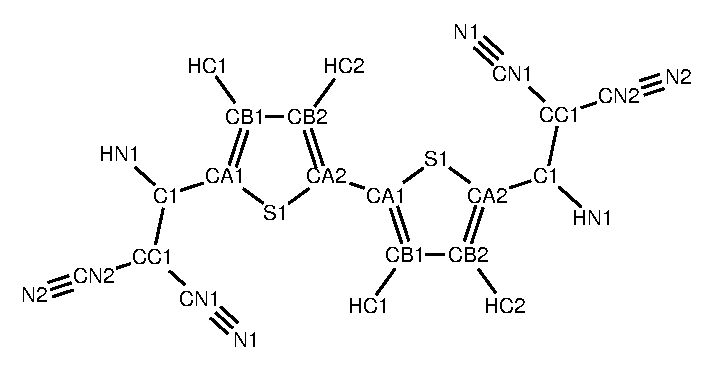
\includegraphics[width=0.45\textwidth]{./fig/chemical_structure/dcv2t_atom_types}\,
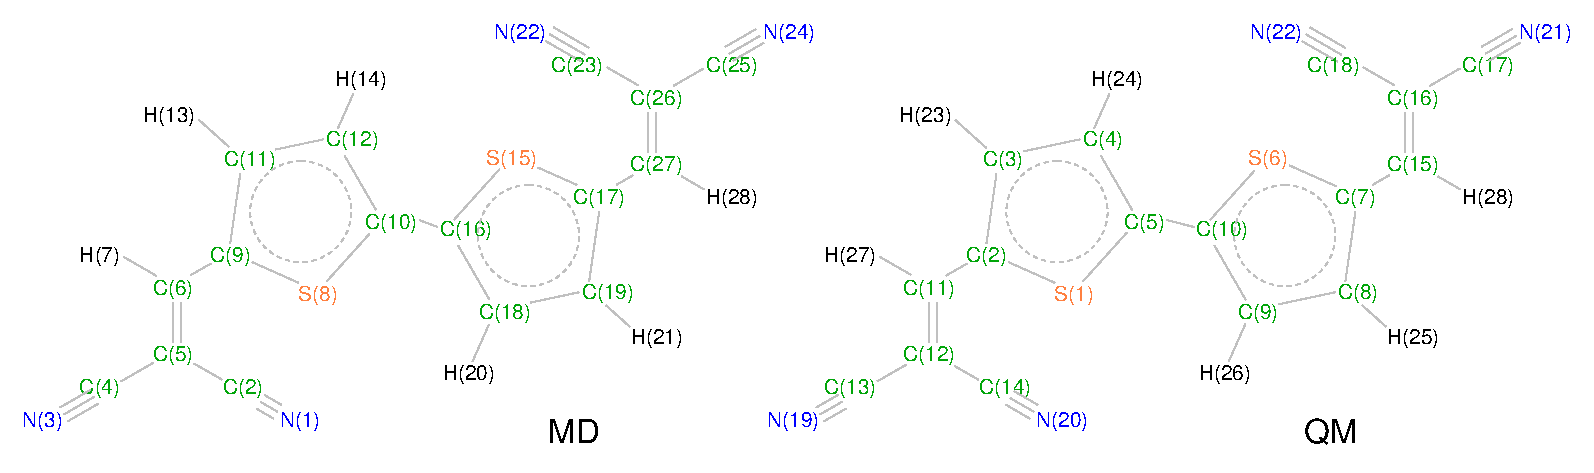
\includegraphics[width=0.45\textwidth]{./fig/chemical_structure/dcv2t_gaussian}
\caption{\small (a) \dcvt with atoms labelled according to \texttt{residue\_number:residue\_name:atom\_name}. There are four residues and two residue types: thiophene (THI) and dicyanovinyl (NIT). The corresponding pdb file is shown in listing~\ref{list:pdb}. (b) Atom numbering is used to split conjugated segments on rigid fragments and to link atomistic and quantum descriptions.}
\label{fig:dcv2t}
\end{figure}

\lstinputlisting[
  language=XML,
  basicstyle=\ttfamily\footnotesize,
  stringstyle=\ttfamily\footnotesize,
  showstringspaces=false,
  frame=lines,
  label=list:pdb, 
  morekeywords={HETATM,THI,NIT},
  caption={\small pdb file of \dcvt.}]%
{./fig/chemical_structure/dcv2t.pdb}

\section{Mapping file}
\label{sec:xmlmap}

The mapping file (referred here as \xmlcsg) is used by the program \ctpmap to convert an atomistic trajectory to a coarse-grained one. The coarse-grained trajectory contains positions, names, types, and orientations of rigid fragments. \xmlcsg contains definitions of rigid fragments (coarse-grained beads) and identifies to what conjugated segment a particular rigid fragment belongs. The description of the mapping options is given in table \ref{tab:map}. An example of \xmlcsg for a \dcvt molecule is shown in listing~\ref{list:map}. 

\begin{table}[ht]
\label{tab:map}
\caption{Description of the \xml mapping file (\xmlcsg).}
\rowcolors{1}{invisiblegray}{white} {\footnotesize \input{reference/xml/map.xml}}
\end{table}
\vfill
% Define new language for listings.
\lstdefinelanguage{MXML} {
   basicstyle=\ttfamily\scriptsize,
   sensitive=true,
   morecomment=[s][\color{gray}\rmfamily\itshape]{<!--}{-->}, 
   showstringspaces=false,
   numberstyle=\scriptsize,
   numberblanklines=true,
   showspaces=false,
   breaklines=true,
   showtabs=false,
   alsoletter={:},
   keywords = [1]
   { name,cg_molecule,cg_beads,cg_bead,crgunitname,bead,beads,type,topology,name,ident,maps,map,mapping,weights,position,qm,symmetry },
   keywordstyle={[1]\color{blue}},
}
\lstinputlisting[
 language=MXML,
 label=list:map,
 caption={Examle of \xmlcsg for \dcvt. Each rigid fragment (coarse-grained bead) is defined by a list of atoms. Atom numbers, names, and residue names should correspond to those used in \gromacs topology (see the corresponing listing \ref{list:pdb} of the pdb file).}]%
{./input/dcv2t/map.xml}

\clearpage
\section{Conjugated segments and rigid fragments}

Conjugated segments are described in a separate \xml file. An example for \dcvt is shown in listing~\ref{list:conjugated_segments}.



\clearpage
\begin{figure}[ht]
\centering
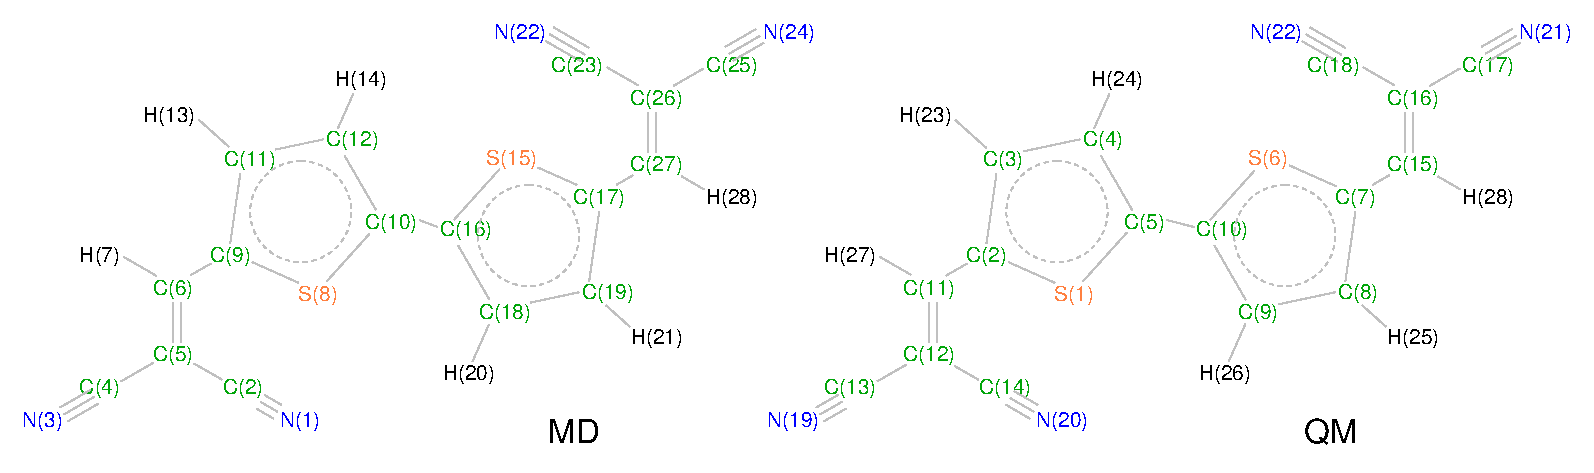
\includegraphics[width=\textwidth]{./fig/chemical_structure/dcv2t_gaussian} 
\caption{\small Atom order of \dcvt in the atomistic topology (MD) and qunatum chemical calculations (QM). The  link between two is established in the description of a conjugated segment shown in listing~\ref{list:conjugated_segments}.}
\label{fig:dcv2t_qm}
\end{figure}

\lstset{
  language=XML,
  frame=lines,
  basicstyle=\ttfamily\footnotesize,
  identifierstyle=\color{red},
  keywordstyle=\color{blue},
  showstringspaces=false,
  columns=fullflexible,
  commentstyle=\color{gray}\rmfamily\itshape,
  morekeywords={crgunit_type,ChargeUnitType,posname,orbname,basisset,transorb,reorg,nameneutr,namecrg,energy,beadconj,molname,name,monomer_atom_map,monomer_atom_weights},
}

\lstinputlisting[
 label=list:conjugated_segments, 
 caption={\small \xml file describing conjugated segments.
}]%
{./input/segments.xml}
\clearpage


\section{Molecular orbitals}
If the semi-empirical method is used to calculate electronic coupling elements, molecular orbitals of all molecules must be supplied. They can be generated using \gaussian program. The \gaussian input file for \dcvt is shown in listing~\ref{list:zindo_orbitals}. Provided with this input, \gaussian will generate \texttt{fort.7} file which contains the molecular orbitals of a \dcvt. This file can be renamed to \texttt{\dcvt.orb}. Note that the order of the atoms in the input file and the order of coefficients should always match. Therefore, the coordinate part of the input file must be supplied together with the orbitals. We will assume the coordinates, in the format \texttt{atom\_type: x y z}, is saved to the \texttt{\dcvt.xyz} file.

\attention{Izindo requires the specification of orbitals for hole and electron transport in \xmlcsg. They are the HOMO and LUMO respectively and can be retrieved from the \texttt{log} file from which the \texttt{\dcvt.orb} file is generated. The number of \texttt{alpha electrons} is the HOMO, the LUMO is HOMO+1 } 

\lstinputlisting[
 label=list:zindo_orbitals, 
 basicstyle=\ttfamily\footnotesize,
 morekeywords={chk,mem,punch,int,S,C,S,N,H},
 showstringspaces=false,
 keepspaces=true,
 caption={\small \gaussian input file \texttt{get\_orbitals.com} used for generating molecular orbitals. The first line contains  the name of the check file, the second the requested RAM. 
%
 \texttt{int=zindos} requests the method ZINDO, \texttt{punch=mo} states that the molecular orbitals ought to be written to  the \texttt{fort.7} file, \texttt{nosymm} forbids use of symmetry and is necessary to ensure correct position of orbitals with respect to the provided coordinates. The two integer numbers correspond to the charge and multiplicity of the system: $0\, 1$ corresponds to a neutral system with a multiplicity of one. They are followed by the types and coordinates of all atoms in the molecule.
}]%
{./input/get_orbitals.com}
%


\section{DFT transfer integrals}
\lstinputlisting[
  language=XML,
  label=list:TI_xml,
  stringstyle=\ttfamily\footnotesize,
  showstringspaces=false,
  caption={\small Example {\tt TI.xml} file created as the output of a \dipro calculation. Due to slightly different implementations, the orbitals indices refer to monomer indices in a \gaussian run but to indices in the merged dimer guess in a \turbomole run.}] {./input/TI.xml}




\chapter{Programs and interfaces}
\section{Programs}
\newcommand{\integrals}{\hyperref[calc:integrals]{\texttt{integrals}}\xspace}

\subsection{Molecular Orbital Overlap}

\moo can be used both in a sandalone mode and as a \calculator of the \votcact. \moo constructs the Fock operator of a dimer from the  molecular orbitals of monomers by translating and rotating the orbitals and therefore requires the optimized geometry of the molecule and the projection coefficients of the molecular on atomic orbitals. 


\subsubsection{Standalone use}
MOO can also be used in a standalone mode. For this purpose a program \overlap is provided 
\begin{verbatim}
 moo_overlap --conjseg benzene.xml --pos1 benzene1.pos --pos2 benzene2.pos
\end{verbatim}
Its input requires a description of two conjugated segments (\texttt{benzene.xml}, positions and orientations of the molecules and the files with molecular coordinates and orbitals. The structure of the files is shown in listings \ref{list:benzene_xml} and  \ref{list:benzene_pos}.
\vskip 0.1cm
\lstinputlisting[label=list:benzene_xml,caption={\small \texttt{benzene.xml} file with the description of the benzene molecule, which is also a single conjugated segment and a rigid fragment.}] {./fig/moo/moo_overlap/benzene.xml}
\vskip 0.1cm
\lstinputlisting[label=list:benzene_pos, caption={\small \texttt{benzene1.pos} file which describes the position and orientation of the molecule. The name of the molecule is followed by three coordinates (relative to the center of mass of the supplied \texttt{xyz} file and then by nine elements of the rotation matrix $a_{ij} = e_i e^\text{mol}_j $. The reference coordinate frame is determined from the provided \texttt{xyz} file.}] {./fig/moo/moo_overlap/benzene1.pos}


\subsubsection{Calculator of \votcact}
Semi-empirical method of evaluation of electronic couplings is provided by the \integrals calculator of  \ctprun
\begin{verbatim}
  ctp_run --exec "intergals"
\end{verbatim}


\moo requires the following input files: \\
\noindent
\xyz contains four columns, first being the atom type and the next three its coordinates. This is a standard \texttt{xyz} format without a header. 
\vskip 0.1cm
\noindent

\subsubsection{Molecular orbitals}
\orb can be generated using \gaussian program and the input script \texttt{get\_orbitals.com} which shown in listing~\ref{list:zindo_orbitals}.
\vskip 0.1cm
\noindent
\lstinputlisting[
 label=list:zindo_orbitals, 
 caption={\footnotesize \gaussian input file \texttt{get\_orbitals.com} used for generating molecular orbitals. The first line contains  the name of the check file, the second the requested RAM. 
%
 \texttt{int=zindos} requests the method ZINDO, \texttt{punch=mo} states that the molecular orbitals ought to be written to  the \texttt{fort.7} file, \texttt{nosymm} forbids use of symmetry and is necessary to ensure correct position of orbitals with respect to the provided coordinates. The two integer numbers correspond to the charge and multiplicity of the system: $0\, 1$ corresponds to a neutral system with a multiplicity of one. They are followed by the types and coordinates of all atoms in the molecule.
}]%
{./fig/moo/get_orbitals.com}
%
Provided with this input, \gaussian will generate \texttt{fort.7} file containing the molecular orbitals of a single molecule. This file can be renamed to \orb. 


\subsection{Calculators}
\label{sec:calculators}

Calculator is a piece of code which computes specific system properties, such as site energies, transfer integrals, etc. \ctprun is a wrapper program which executes all calculators. The generic syntax is 
\begin{verbatim}
  ctp_run --exec "calc1, calc2, ..." --opt options.xml
\end{verbatim}
%
File \texttt{options.xml} lists all options needed to run a specific calculator. The format of this file is explained in listing~\ref{list:calc}. A complete list of calculators is given in the \refcalc reference section.
%
\lstinputlisting[label=list:calc, 
 caption={\small A part of the \texttt{options.xml} file with options for the \texttt{calculator\_name\{1,2\}} \refcalc.
}]{./programs/calculators.xml}


\section{Interfaces}

\subsection{Density-functional method}

\begin{itemize}
\item {\it not sure about directory structure yet, using {\tt
      \$DIRECTORY} for the time being}
\item creating file structure for frame $N$ (raw: no postpocessing,
  min: MD energy minimization) in directory {\tt OUTDIR}
\begin{verbatim}
$DIRECTORY/perpare.sh raw/min N OUTDIR
cd OUTDIR
$DIRECTORY/pairdump.sh
\end{verbatim}
\item make sure QCP environments are set!
\item running calculations for all monomers
 \begin{verbatim}
$DIRECTORY/calc_monomer QCP [METHOD]

QCP:   G for Gaussian09
       T for Turbomole

METHOD: func/basis (optional)
        overrides default functional/basisset combination
        defaults: pbepbe/6-311G** Gaussian09
                  b-p/def-TZVP    Turbomole
\end{verbatim}
\item check monomer calculations (Gaussian version to test!) 
\begin{verbatim}
$DIRECTORY/check_mols N M QCP

N:   First monomer to test
M:   Last monomer to test
QCP: G/T 
\end{verbatim}
incomplete monomers are written to file {\tt TROUBLE.mol}
\item running calculations for all dimers
 \begin{verbatim}
$DIRECTORY/calc_dimer_noSCF QCP [METHOD]

QCP:   G for Gaussian09
       T for Turbomole

METHOD: func/basis (optional)
        overrides default functional/basisset combination
        defaults: pbepbe/6-311G** Gaussian09
                  b-p/def-TZVP    Turbomole
\end{verbatim}
\item should we add {\tt trajectory\_submit.sh} that does all monomer
  and dimer calculations on the cluster (MPIP-specific)?
\end{itemize}

\chapter{Manual pages}

\section{Programs}
\label{ref:programs}
\input{reference/programs/all}

\section{Calculators}
\label{ref:caclulators}
\input{reference/calculators/all}

\section{Options}
\label{ref:options}
\input{reference/xml/ctp_listcharges.xml}



\bibliographystyle{achemso}
\bibliography{literature_short}

\end{document} 
